 \documentclass{article}
\usepackage[utf8]{inputenc}
\usepackage[a4paper, total={7in, 10in}]{geometry}
\usepackage{braket}
\usepackage{xcolor}
\usepackage{amsmath}
\usepackage{amssymb}
\usepackage{amsfonts}
\usepackage{graphicx}
\usepackage{svg}
\usepackage{float}
\usepackage{tikz}
\usepackage[ruled,vlined]{algorithm2e}
\usepackage{multicol}
\usepackage[backend=biber,style=alphabetic,sorting=ynt]{biblatex}
\usepackage{xcolor}
%\addbibresource{sample.bib} %Import the bibliography file

\newcommand{\commentt}[1]{\textcolor{blue}{ \textbf{[COMMENT]} #1}}
\newcommand{\ctt}[1]{\commentt{#1}}
\newcommand{\prb}[1]{ \mathbf{Pr} \left[ {#1} \right]}
\newcommand{\onotation}[1]{\(\mathcal{O} \left( {#1}  \right) \)}
\newcommand{\ona}[1]{\onotation{#1}}
\newcommand{\PSI}{{\ket{\psi}}}
\newcommand{\LESn}{\ket{\psi_n}}
\newcommand{\LESa}{\ket{\phi_n}}
\newcommand{\LESs}{\frac{1}{\sqrt{n}}\sum_{i}{\ket{\left(0^{i}10^{n-i}\right)^{n}}}}
\newcommand{\Hn}{\mathcal{H}_{n}}
\newcommand{\Ep}{\frac{1}{\sqrt{2^n}}\sum^{2^n}_{x}{ \ket{xx}}}
\newcommand{\HON}{\ket{\psi_{\text{honest}}}}
\newcommand{\Lemma}{\paragraph{Lemma.}}


\setlength{\columnsep}{0.6cm}

\newcommand{\Gz}{ G_{z}^{\delta} } 

\begin{document}

\title{Quantum LTC With Positive Rate}
\author{David Ponarovsky}
\maketitle
\begin{multicols*}{2}
\newcommand{ \Hw }{ \delta\Delta -\Delta^{\frac{1}{2}-\varepsilon}/\delta  }
	\newcommand{ \Nw }{ \Delta^{\frac{3}{2}-\varepsilon}} 
	  \newcommand{ \Gu } { \Gamma^{\cup} }
	  \newcommand{ \Guq } { \Gamma^{\cup, \square} }

    	\newcommand{ \Gsa } {\Gamma_{\square_{1}} }
	\newcommand{ \Gsb } {\Gamma_{\square_{2}} }
        \newcommand{ \Aa } { C_{A_{1}}}  
	\newcommand{ \Ab } { C_{A_{2}}}
	\newcommand{ \Ac } { C_{A_{3}}}
	\newcommand{ \Aab } { \Aa \otimes \Ab } 
	\newcommand{ \Aac } { \Aa \otimes \Ac }
	\newcommand{ \Aabc } { \Aa \otimes \Ab \otimes \Ac }
	\newcommand{ \Aabp } { \Aa^{\perp} \otimes \Ab^{\perp} } 
	\newcommand{ \Aacp } { \Aa^{\perp} \otimes \Ac^{\perp} }
	\newcommand{ \Aabcp } { \Aa^{\perp} \otimes \Ab^{\perp} \otimes \Ac^{\perp} }
	\newcommand{ \Aabpp } { \left( \Aabp \right)^\perp } 
	\newcommand{ \Aacpp } { \left( \Aacp \right)^\perp }
	\newcommand{ \Aabcpp } { \left( \Aabcp \right)^\perp }
	\newcommand{ \YY } {  y_{1}y_{2}^{\top} }
	\newcommand{ \ZZ } {  z_{1}z_{2}^{\top} } 
	\newcommand{ \TT } { \tilde{\tau} } 


  \paragraph{preamble.} preamble.  
  \begin{figure}[H]
            %\label{fig:square}
            \begin{center}
            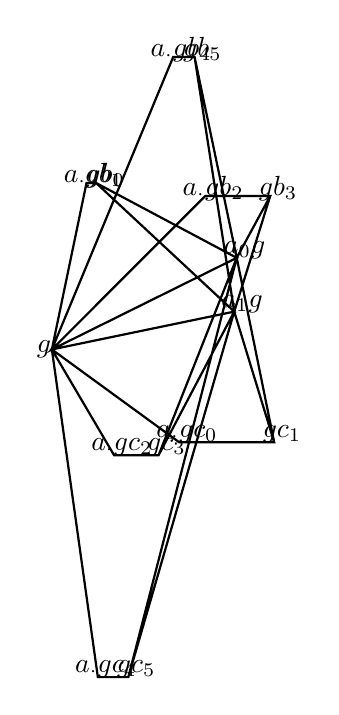
\begin{tikzpicture}
            \draw[thick](0,0)(0,0)  -- (0.43991388380350016, 2.1143211438786547) -- (0.5614774738058519, 2.1143211438786547) -- (2.347785915894221,1.1637459452711834) -- (0,0) -- (0,0)  -- (1.6168988353997729, -1.1784558206947882) -- (2.823427689773725, -1.1784558206947882) -- (2.347785915894221,1.1637459452711834) -- (0,0) -- 
(0,0)  -- (0.43991388380350016, 2.1143211438786547) -- (0.5614774738058519, 2.1143211438786547) -- (2.347785915894221,1.1637459452711834) -- (0,0) -- (0,0)  -- (0.7899633068769163, -1.3428973265950472) -- (1.3553894712977759, -1.3428973265950472) -- (2.347785915894221,1.1637459452711834) -- (0,0) -- 
(0,0)  -- (0.43991388380350016, 2.1143211438786547) -- (0.5614774738058519, 2.1143211438786547) -- (2.347785915894221,1.1637459452711834) -- (0,0) -- (0,0)  -- (0.5839090175886481, -4.161209429857939) -- (0.9709961218224361, -4.161209429857939) -- (2.347785915894221,1.1637459452711834) -- (0,0) -- 
(0,0)  -- (1.9481489256792388, 1.9489393164693114) -- (2.7731683840594963, 1.9489393164693114) -- (2.347785915894221,1.1637459452711834) -- (0,0) -- (0,0)  -- (1.6168988353997729, -1.1784558206947882) -- (2.823427689773725, -1.1784558206947882) -- (2.347785915894221,1.1637459452711834) -- (0,0) -- 
(0,0)  -- (1.9481489256792388, 1.9489393164693114) -- (2.7731683840594963, 1.9489393164693114) -- (2.347785915894221,1.1637459452711834) -- (0,0) -- (0,0)  -- (0.7899633068769163, -1.3428973265950472) -- (1.3553894712977759, -1.3428973265950472) -- (2.347785915894221,1.1637459452711834) -- (0,0) -- 
(0,0)  -- (1.9481489256792388, 1.9489393164693114) -- (2.7731683840594963, 1.9489393164693114) -- (2.347785915894221,1.1637459452711834) -- (0,0) -- (0,0)  -- (0.5839090175886481, -4.161209429857939) -- (0.9709961218224361, -4.161209429857939) -- (2.347785915894221,1.1637459452711834) -- (0,0) -- 
(0,0)  -- (1.5404344886618306, 3.71340587071375) -- (1.8127201886730941, 3.71340587071375) -- (2.347785915894221,1.1637459452711834) -- (0,0) -- (0,0)  -- (1.6168988353997729, -1.1784558206947882) -- (2.823427689773725, -1.1784558206947882) -- (2.347785915894221,1.1637459452711834) -- (0,0) -- 
(0,0)  -- (1.5404344886618306, 3.71340587071375) -- (1.8127201886730941, 3.71340587071375) -- (2.347785915894221,1.1637459452711834) -- (0,0) -- (0,0)  -- (0.7899633068769163, -1.3428973265950472) -- (1.3553894712977759, -1.3428973265950472) -- (2.347785915894221,1.1637459452711834) -- (0,0) -- 
(0,0)  -- (1.5404344886618306, 3.71340587071375) -- (1.8127201886730941, 3.71340587071375) -- (2.347785915894221,1.1637459452711834) -- (0,0) -- (0,0)  -- (0.5839090175886481, -4.161209429857939) -- (0.9709961218224361, -4.161209429857939) -- (2.347785915894221,1.1637459452711834) -- (0,0) -- 
(0,0)  -- (0.43991388380350016, 2.1143211438786547) -- (0.5614774738058519, 2.1143211438786547) -- (2.3159604027707923,0.4807189220030325) -- (0,0) -- (0,0)  -- (1.6168988353997729, -1.1784558206947882) -- (2.823427689773725, -1.1784558206947882) -- (2.3159604027707923,0.4807189220030325) -- (0,0) -- 
(0,0)  -- (0.43991388380350016, 2.1143211438786547) -- (0.5614774738058519, 2.1143211438786547) -- (2.3159604027707923,0.4807189220030325) -- (0,0) -- (0,0)  -- (0.7899633068769163, -1.3428973265950472) -- (1.3553894712977759, -1.3428973265950472) -- (2.3159604027707923,0.4807189220030325) -- (0,0) -- 
(0,0)  -- (0.43991388380350016, 2.1143211438786547) -- (0.5614774738058519, 2.1143211438786547) -- (2.3159604027707923,0.4807189220030325) -- (0,0) -- (0,0)  -- (0.5839090175886481, -4.161209429857939) -- (0.9709961218224361, -4.161209429857939) -- (2.3159604027707923,0.4807189220030325) -- (0,0) -- 
(0,0)  -- (1.9481489256792388, 1.9489393164693114) -- (2.7731683840594963, 1.9489393164693114) -- (2.3159604027707923,0.4807189220030325) -- (0,0) -- (0,0)  -- (1.6168988353997729, -1.1784558206947882) -- (2.823427689773725, -1.1784558206947882) -- (2.3159604027707923,0.4807189220030325) -- (0,0) -- 
(0,0)  -- (1.9481489256792388, 1.9489393164693114) -- (2.7731683840594963, 1.9489393164693114) -- (2.3159604027707923,0.4807189220030325) -- (0,0) -- (0,0)  -- (0.7899633068769163, -1.3428973265950472) -- (1.3553894712977759, -1.3428973265950472) -- (2.3159604027707923,0.4807189220030325) -- (0,0) -- 
(0,0)  -- (1.9481489256792388, 1.9489393164693114) -- (2.7731683840594963, 1.9489393164693114) -- (2.3159604027707923,0.4807189220030325) -- (0,0) -- (0,0)  -- (0.5839090175886481, -4.161209429857939) -- (0.9709961218224361, -4.161209429857939) -- (2.3159604027707923,0.4807189220030325) -- (0,0) -- 
(0,0)  -- (1.5404344886618306, 3.71340587071375) -- (1.8127201886730941, 3.71340587071375) -- (2.3159604027707923,0.4807189220030325) -- (0,0) -- (0,0)  -- (1.6168988353997729, -1.1784558206947882) -- (2.823427689773725, -1.1784558206947882) -- (2.3159604027707923,0.4807189220030325) -- (0,0) -- 
(0,0)  -- (1.5404344886618306, 3.71340587071375) -- (1.8127201886730941, 3.71340587071375) -- (2.3159604027707923,0.4807189220030325) -- (0,0) -- (0,0)  -- (0.7899633068769163, -1.3428973265950472) -- (1.3553894712977759, -1.3428973265950472) -- (2.3159604027707923,0.4807189220030325) -- (0,0) -- 
(0,0)  -- (1.5404344886618306, 3.71340587071375) -- (1.8127201886730941, 3.71340587071375) -- (2.3159604027707923,0.4807189220030325) -- (0,0) -- (0,0)  -- (0.5839090175886481, -4.161209429857939) -- (0.9709961218224361, -4.161209429857939) -- (2.3159604027707923,0.4807189220030325) -- (0,0) -- 
(0,0);
\node at (-0.1,0) {$ g $};
\node at (2.447785915894221,1.2637459452711834) {$ a_{ 0 }g $};
\node at (2.4159604027707924,0.5807189220030325) {$ a_{ 1 }g $};
\node at (0.5399138838035001,2.2143211438786548) {$ a_{\cdot} gb_{ 0 } $};
\node at (0.6614774738058519,2.2143211438786548) {$ gb_{ 1 } $};
\node at (2.048148925679239,2.0489393164693115) {$ a_{\cdot} gb_{ 2 } $};
\node at (2.8731683840594964,2.0489393164693115) {$ gb_{ 3 } $};
\node at (1.6404344886618307,3.81340587071375) {$ a_{\cdot} gb_{ 4 } $};
\node at (1.9127201886730942,3.81340587071375) {$ gb_{ 5 } $};
\node at (1.716898835399773,-1.078455820694788) {$ a_{\cdot} gc_{ 0 } $};
\node at (2.923427689773725,-1.078455820694788) {$ gc_{ 1 } $};
\node at (0.8899633068769163,-1.2428973265950471) {$ a_{\cdot} gc_{ 2 } $};
\node at (1.455389471297776,-1.2428973265950471) {$ gc_{ 3 } $};
\node at (0.6839090175886481,-4.061209429857939) {$ a_{\cdot} gc_{ 4 } $};
\node at (1.0709961218224362,-4.061209429857939) {$ gc_{ 5 } $};

            \end{tikzpicture}
            \end{center}
            \caption{Square of the complex, with edges $(g,ag), (agb, gb) \in E_A,
            (g,gb), (agb, ag) \in E_B.$ \label{fig:square}
            }
            \end{figure}
 \begin{figure}[H]
            %\label{fig:square}
            \begin{center}
            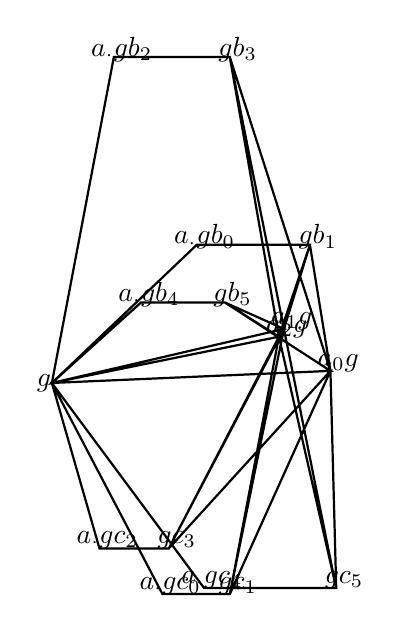
\begin{tikzpicture}
            \draw[thick](0,0)(0,0)  -- (1.8396770558134976, 1.7540239725897262) -- (3.2771376992550603, 1.7540239725897262) -- (3.5377282402428025,0.1536004304065323) -- (0,0) -- (0,0)  -- (1.4039393581529467, -2.680089295477668) -- (2.2607251072016616, -2.680089295477668) -- (3.5377282402428025,0.1536004304065323) -- (0,0) -- 
(0,0)  -- (1.8396770558134976, 1.7540239725897262) -- (3.2771376992550603, 1.7540239725897262) -- (3.5377282402428025,0.1536004304065323) -- (0,0) -- (0,0)  -- (0.604345703750544, -2.1012051485648056) -- (1.4854846701491533, -2.1012051485648056) -- (3.5377282402428025,0.1536004304065323) -- (0,0) -- 
(0,0)  -- (1.8396770558134976, 1.7540239725897262) -- (3.2771376992550603, 1.7540239725897262) -- (3.5377282402428025,0.1536004304065323) -- (0,0) -- (0,0)  -- (1.9333113616574227, -2.6051427108163194) -- (3.611158399682563, -2.6051427108163194) -- (3.5377282402428025,0.1536004304065323) -- (0,0) -- 
(0,0)  -- (0.7870348968045164, 4.138756293913056) -- (2.259871197610281, 4.138756293913056) -- (3.5377282402428025,0.1536004304065323) -- (0,0) -- (0,0)  -- (1.4039393581529467, -2.680089295477668) -- (2.2607251072016616, -2.680089295477668) -- (3.5377282402428025,0.1536004304065323) -- (0,0) -- 
(0,0)  -- (0.7870348968045164, 4.138756293913056) -- (2.259871197610281, 4.138756293913056) -- (3.5377282402428025,0.1536004304065323) -- (0,0) -- (0,0)  -- (0.604345703750544, -2.1012051485648056) -- (1.4854846701491533, -2.1012051485648056) -- (3.5377282402428025,0.1536004304065323) -- (0,0) -- 
(0,0)  -- (0.7870348968045164, 4.138756293913056) -- (2.259871197610281, 4.138756293913056) -- (3.5377282402428025,0.1536004304065323) -- (0,0) -- (0,0)  -- (1.9333113616574227, -2.6051427108163194) -- (3.611158399682563, -2.6051427108163194) -- (3.5377282402428025,0.1536004304065323) -- (0,0) -- 
(0,0)  -- (1.133308785603062, 1.0230034233741332) -- (2.1956322772893797, 1.0230034233741332) -- (3.5377282402428025,0.1536004304065323) -- (0,0) -- (0,0)  -- (1.4039393581529467, -2.680089295477668) -- (2.2607251072016616, -2.680089295477668) -- (3.5377282402428025,0.1536004304065323) -- (0,0) -- 
(0,0)  -- (1.133308785603062, 1.0230034233741332) -- (2.1956322772893797, 1.0230034233741332) -- (3.5377282402428025,0.1536004304065323) -- (0,0) -- (0,0)  -- (0.604345703750544, -2.1012051485648056) -- (1.4854846701491533, -2.1012051485648056) -- (3.5377282402428025,0.1536004304065323) -- (0,0) -- 
(0,0)  -- (1.133308785603062, 1.0230034233741332) -- (2.1956322772893797, 1.0230034233741332) -- (3.5377282402428025,0.1536004304065323) -- (0,0) -- (0,0)  -- (1.9333113616574227, -2.6051427108163194) -- (3.611158399682563, -2.6051427108163194) -- (3.5377282402428025,0.1536004304065323) -- (0,0) -- 
(0,0)  -- (1.8396770558134976, 1.7540239725897262) -- (3.2771376992550603, 1.7540239725897262) -- (2.9471715066876287,0.6861398747179884) -- (0,0) -- (0,0)  -- (1.4039393581529467, -2.680089295477668) -- (2.2607251072016616, -2.680089295477668) -- (2.9471715066876287,0.6861398747179884) -- (0,0) -- 
(0,0)  -- (1.8396770558134976, 1.7540239725897262) -- (3.2771376992550603, 1.7540239725897262) -- (2.9471715066876287,0.6861398747179884) -- (0,0) -- (0,0)  -- (0.604345703750544, -2.1012051485648056) -- (1.4854846701491533, -2.1012051485648056) -- (2.9471715066876287,0.6861398747179884) -- (0,0) -- 
(0,0)  -- (1.8396770558134976, 1.7540239725897262) -- (3.2771376992550603, 1.7540239725897262) -- (2.9471715066876287,0.6861398747179884) -- (0,0) -- (0,0)  -- (1.9333113616574227, -2.6051427108163194) -- (3.611158399682563, -2.6051427108163194) -- (2.9471715066876287,0.6861398747179884) -- (0,0) -- 
(0,0)  -- (0.7870348968045164, 4.138756293913056) -- (2.259871197610281, 4.138756293913056) -- (2.9471715066876287,0.6861398747179884) -- (0,0) -- (0,0)  -- (1.4039393581529467, -2.680089295477668) -- (2.2607251072016616, -2.680089295477668) -- (2.9471715066876287,0.6861398747179884) -- (0,0) -- 
(0,0)  -- (0.7870348968045164, 4.138756293913056) -- (2.259871197610281, 4.138756293913056) -- (2.9471715066876287,0.6861398747179884) -- (0,0) -- (0,0)  -- (0.604345703750544, -2.1012051485648056) -- (1.4854846701491533, -2.1012051485648056) -- (2.9471715066876287,0.6861398747179884) -- (0,0) -- 
(0,0)  -- (0.7870348968045164, 4.138756293913056) -- (2.259871197610281, 4.138756293913056) -- (2.9471715066876287,0.6861398747179884) -- (0,0) -- (0,0)  -- (1.9333113616574227, -2.6051427108163194) -- (3.611158399682563, -2.6051427108163194) -- (2.9471715066876287,0.6861398747179884) -- (0,0) -- 
(0,0)  -- (1.133308785603062, 1.0230034233741332) -- (2.1956322772893797, 1.0230034233741332) -- (2.9471715066876287,0.6861398747179884) -- (0,0) -- (0,0)  -- (1.4039393581529467, -2.680089295477668) -- (2.2607251072016616, -2.680089295477668) -- (2.9471715066876287,0.6861398747179884) -- (0,0) -- 
(0,0)  -- (1.133308785603062, 1.0230034233741332) -- (2.1956322772893797, 1.0230034233741332) -- (2.9471715066876287,0.6861398747179884) -- (0,0) -- (0,0)  -- (0.604345703750544, -2.1012051485648056) -- (1.4854846701491533, -2.1012051485648056) -- (2.9471715066876287,0.6861398747179884) -- (0,0) -- 
(0,0)  -- (1.133308785603062, 1.0230034233741332) -- (2.1956322772893797, 1.0230034233741332) -- (2.9471715066876287,0.6861398747179884) -- (0,0) -- (0,0)  -- (1.9333113616574227, -2.6051427108163194) -- (3.611158399682563, -2.6051427108163194) -- (2.9471715066876287,0.6861398747179884) -- (0,0) -- 
(0,0)  -- (1.8396770558134976, 1.7540239725897262) -- (3.2771376992550603, 1.7540239725897262) -- (2.8836763542470427,0.5872663129498827) -- (0,0) -- (0,0)  -- (1.4039393581529467, -2.680089295477668) -- (2.2607251072016616, -2.680089295477668) -- (2.8836763542470427,0.5872663129498827) -- (0,0) -- 
(0,0)  -- (1.8396770558134976, 1.7540239725897262) -- (3.2771376992550603, 1.7540239725897262) -- (2.8836763542470427,0.5872663129498827) -- (0,0) -- (0,0)  -- (0.604345703750544, -2.1012051485648056) -- (1.4854846701491533, -2.1012051485648056) -- (2.8836763542470427,0.5872663129498827) -- (0,0) -- 
(0,0)  -- (1.8396770558134976, 1.7540239725897262) -- (3.2771376992550603, 1.7540239725897262) -- (2.8836763542470427,0.5872663129498827) -- (0,0) -- (0,0)  -- (1.9333113616574227, -2.6051427108163194) -- (3.611158399682563, -2.6051427108163194) -- (2.8836763542470427,0.5872663129498827) -- (0,0) -- 
(0,0)  -- (0.7870348968045164, 4.138756293913056) -- (2.259871197610281, 4.138756293913056) -- (2.8836763542470427,0.5872663129498827) -- (0,0) -- (0,0)  -- (1.4039393581529467, -2.680089295477668) -- (2.2607251072016616, -2.680089295477668) -- (2.8836763542470427,0.5872663129498827) -- (0,0) -- 
(0,0)  -- (0.7870348968045164, 4.138756293913056) -- (2.259871197610281, 4.138756293913056) -- (2.8836763542470427,0.5872663129498827) -- (0,0) -- (0,0)  -- (0.604345703750544, -2.1012051485648056) -- (1.4854846701491533, -2.1012051485648056) -- (2.8836763542470427,0.5872663129498827) -- (0,0) -- 
(0,0)  -- (0.7870348968045164, 4.138756293913056) -- (2.259871197610281, 4.138756293913056) -- (2.8836763542470427,0.5872663129498827) -- (0,0) -- (0,0)  -- (1.9333113616574227, -2.6051427108163194) -- (3.611158399682563, -2.6051427108163194) -- (2.8836763542470427,0.5872663129498827) -- (0,0) -- 
(0,0)  -- (1.133308785603062, 1.0230034233741332) -- (2.1956322772893797, 1.0230034233741332) -- (2.8836763542470427,0.5872663129498827) -- (0,0) -- (0,0)  -- (1.4039393581529467, -2.680089295477668) -- (2.2607251072016616, -2.680089295477668) -- (2.8836763542470427,0.5872663129498827) -- (0,0) -- 
(0,0)  -- (1.133308785603062, 1.0230034233741332) -- (2.1956322772893797, 1.0230034233741332) -- (2.8836763542470427,0.5872663129498827) -- (0,0) -- (0,0)  -- (0.604345703750544, -2.1012051485648056) -- (1.4854846701491533, -2.1012051485648056) -- (2.8836763542470427,0.5872663129498827) -- (0,0) -- 
(0,0)  -- (1.133308785603062, 1.0230034233741332) -- (2.1956322772893797, 1.0230034233741332) -- (2.8836763542470427,0.5872663129498827) -- (0,0) -- (0,0)  -- (1.9333113616574227, -2.6051427108163194) -- (3.611158399682563, -2.6051427108163194) -- (2.8836763542470427,0.5872663129498827) -- (0,0) -- 
(0,0);
\node at (-0.1,0) {$ g $};
\node at (3.6377282402428026,0.2536004304065323) {$ a_{ 0 }g $};
\node at (3.047171506687629,0.7861398747179884) {$ a_{ 1 }g $};
\node at (2.983676354247043,0.6872663129498827) {$ a_{ 2 }g $};
\node at (1.9396770558134977,1.8540239725897263) {$ a_{\cdot} gb_{ 0 } $};
\node at (3.3771376992550604,1.8540239725897263) {$ gb_{ 1 } $};
\node at (0.8870348968045164,4.238756293913056) {$ a_{\cdot} gb_{ 2 } $};
\node at (2.359871197610281,4.238756293913056) {$ gb_{ 3 } $};
\node at (1.233308785603062,1.1230034233741333) {$ a_{\cdot} gb_{ 4 } $};
\node at (2.29563227728938,1.1230034233741333) {$ gb_{ 5 } $};
\node at (1.5039393581529468,-2.5800892954776677) {$ a_{\cdot} gc_{ 0 } $};
\node at (2.3607251072016617,-2.5800892954776677) {$ gc_{ 1 } $};
\node at (0.704345703750544,-2.0012051485648055) {$ a_{\cdot} gc_{ 2 } $};
\node at (1.5854846701491534,-2.0012051485648055) {$ gc_{ 3 } $};
\node at (2.0333113616574225,-2.5051427108163193) {$ a_{\cdot} gc_{ 4 } $};
\node at (3.7111583996825632,-2.5051427108163193) {$ gc_{ 5 } $};

            \end{tikzpicture}
            \end{center}
            \caption{Square of the complex, with edges $(g,ag), (agb, gb) \in E_A,
            (g,gb), (agb, ag) \in E_B.$ \label{fig:square}
            }
            \end{figure}
 \begin{figure}[H]
            %\label{fig:square}
            \begin{center}
            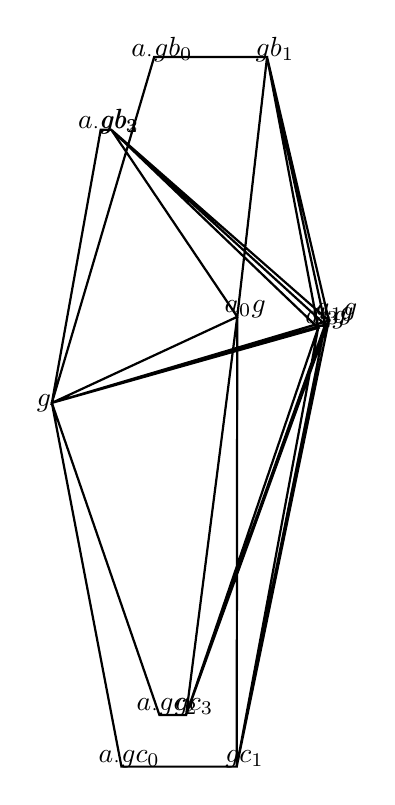
\begin{tikzpicture}
            \draw[thick](0,0)(0,0)  -- (1.2987778572270403, 4.391980565392721) -- (2.7328767393412736, 4.391980565392721) -- (2.354417796532394,1.0935589492726312) -- (0,0) -- (0,0)  -- (0.8836892323403085, -4.619489840765112) -- (2.3473068767253986, -4.619489840765112) -- (2.354417796532394,1.0935589492726312) -- (0,0) -- 
(0,0)  -- (1.2987778572270403, 4.391980565392721) -- (2.7328767393412736, 4.391980565392721) -- (2.354417796532394,1.0935589492726312) -- (0,0) -- (0,0)  -- (1.3660738143067637, -3.9643501480201153) -- (1.7047804461836151, -3.9643501480201153) -- (2.354417796532394,1.0935589492726312) -- (0,0) -- 
(0,0)  -- (0.6203624871481315, 3.469339580460739) -- (0.754529844143718, 3.469339580460739) -- (2.354417796532394,1.0935589492726312) -- (0,0) -- (0,0)  -- (0.8836892323403085, -4.619489840765112) -- (2.3473068767253986, -4.619489840765112) -- (2.354417796532394,1.0935589492726312) -- (0,0) -- 
(0,0)  -- (0.6203624871481315, 3.469339580460739) -- (0.754529844143718, 3.469339580460739) -- (2.354417796532394,1.0935589492726312) -- (0,0) -- (0,0)  -- (1.3660738143067637, -3.9643501480201153) -- (1.7047804461836151, -3.9643501480201153) -- (2.354417796532394,1.0935589492726312) -- (0,0) -- 
(0,0)  -- (1.2987778572270403, 4.391980565392721) -- (2.7328767393412736, 4.391980565392721) -- (3.5178966311351876,1.0456466401771805) -- (0,0) -- (0,0)  -- (0.8836892323403085, -4.619489840765112) -- (2.3473068767253986, -4.619489840765112) -- (3.5178966311351876,1.0456466401771805) -- (0,0) -- 
(0,0)  -- (1.2987778572270403, 4.391980565392721) -- (2.7328767393412736, 4.391980565392721) -- (3.5178966311351876,1.0456466401771805) -- (0,0) -- (0,0)  -- (1.3660738143067637, -3.9643501480201153) -- (1.7047804461836151, -3.9643501480201153) -- (3.5178966311351876,1.0456466401771805) -- (0,0) -- 
(0,0)  -- (0.6203624871481315, 3.469339580460739) -- (0.754529844143718, 3.469339580460739) -- (3.5178966311351876,1.0456466401771805) -- (0,0) -- (0,0)  -- (0.8836892323403085, -4.619489840765112) -- (2.3473068767253986, -4.619489840765112) -- (3.5178966311351876,1.0456466401771805) -- (0,0) -- 
(0,0)  -- (0.6203624871481315, 3.469339580460739) -- (0.754529844143718, 3.469339580460739) -- (3.5178966311351876,1.0456466401771805) -- (0,0) -- (0,0)  -- (1.3660738143067637, -3.9643501480201153) -- (1.7047804461836151, -3.9643501480201153) -- (3.5178966311351876,1.0456466401771805) -- (0,0) -- 
(0,0)  -- (1.2987778572270403, 4.391980565392721) -- (2.7328767393412736, 4.391980565392721) -- (3.3820620130760046,0.9522521063210789) -- (0,0) -- (0,0)  -- (0.8836892323403085, -4.619489840765112) -- (2.3473068767253986, -4.619489840765112) -- (3.3820620130760046,0.9522521063210789) -- (0,0) -- 
(0,0)  -- (1.2987778572270403, 4.391980565392721) -- (2.7328767393412736, 4.391980565392721) -- (3.3820620130760046,0.9522521063210789) -- (0,0) -- (0,0)  -- (1.3660738143067637, -3.9643501480201153) -- (1.7047804461836151, -3.9643501480201153) -- (3.3820620130760046,0.9522521063210789) -- (0,0) -- 
(0,0)  -- (0.6203624871481315, 3.469339580460739) -- (0.754529844143718, 3.469339580460739) -- (3.3820620130760046,0.9522521063210789) -- (0,0) -- (0,0)  -- (0.8836892323403085, -4.619489840765112) -- (2.3473068767253986, -4.619489840765112) -- (3.3820620130760046,0.9522521063210789) -- (0,0) -- 
(0,0)  -- (0.6203624871481315, 3.469339580460739) -- (0.754529844143718, 3.469339580460739) -- (3.3820620130760046,0.9522521063210789) -- (0,0) -- (0,0)  -- (1.3660738143067637, -3.9643501480201153) -- (1.7047804461836151, -3.9643501480201153) -- (3.3820620130760046,0.9522521063210789) -- (0,0) -- 
(0,0)  -- (1.2987778572270403, 4.391980565392721) -- (2.7328767393412736, 4.391980565392721) -- (3.47124464277164,0.9948553300029078) -- (0,0) -- (0,0)  -- (0.8836892323403085, -4.619489840765112) -- (2.3473068767253986, -4.619489840765112) -- (3.47124464277164,0.9948553300029078) -- (0,0) -- 
(0,0)  -- (1.2987778572270403, 4.391980565392721) -- (2.7328767393412736, 4.391980565392721) -- (3.47124464277164,0.9948553300029078) -- (0,0) -- (0,0)  -- (1.3660738143067637, -3.9643501480201153) -- (1.7047804461836151, -3.9643501480201153) -- (3.47124464277164,0.9948553300029078) -- (0,0) -- 
(0,0)  -- (0.6203624871481315, 3.469339580460739) -- (0.754529844143718, 3.469339580460739) -- (3.47124464277164,0.9948553300029078) -- (0,0) -- (0,0)  -- (0.8836892323403085, -4.619489840765112) -- (2.3473068767253986, -4.619489840765112) -- (3.47124464277164,0.9948553300029078) -- (0,0) -- 
(0,0)  -- (0.6203624871481315, 3.469339580460739) -- (0.754529844143718, 3.469339580460739) -- (3.47124464277164,0.9948553300029078) -- (0,0) -- (0,0)  -- (1.3660738143067637, -3.9643501480201153) -- (1.7047804461836151, -3.9643501480201153) -- (3.47124464277164,0.9948553300029078) -- (0,0) -- 
(0,0);
\node at (-0.1,0) {$ g $};
\node at (2.454417796532394,1.1935589492726313) {$ a_{ 0 }g $};
\node at (3.6178966311351877,1.1456466401771805) {$ a_{ 1 }g $};
\node at (3.4820620130760047,1.052252106321079) {$ a_{ 2 }g $};
\node at (3.57124464277164,1.0948553300029078) {$ a_{ 3 }g $};
\node at (1.3987778572270404,4.491980565392721) {$ a_{\cdot} gb_{ 0 } $};
\node at (2.8328767393412737,4.491980565392721) {$ gb_{ 1 } $};
\node at (0.7203624871481314,3.5693395804607393) {$ a_{\cdot} gb_{ 2 } $};
\node at (0.854529844143718,3.5693395804607393) {$ gb_{ 3 } $};
\node at (0.9836892323403085,-4.519489840765113) {$ a_{\cdot} gc_{ 0 } $};
\node at (2.4473068767253987,-4.519489840765113) {$ gc_{ 1 } $};
\node at (1.4660738143067638,-3.8643501480201152) {$ a_{\cdot} gc_{ 2 } $};
\node at (1.8047804461836152,-3.8643501480201152) {$ gc_{ 3 } $};

            \end{tikzpicture}
            \end{center}
            \caption{Square of the complex, with edges $(g,ag), (agb, gb) \in E_A,
            (g,gb), (agb, ag) \in E_B.$ \label{fig:square}
            }
            \end{figure}
 
\end{multicols*}
  % \printbibliography 
\end{document}

 